%%%%%%%%%%%%%%%%%%%%%%%%%%%%%%%%%%%%%%%%%
% Stylish Article
% LaTeX Template
% Version 2.0 (13/4/14)
%
% This template has been downloaded from:
% http://www.LaTeXTemplates.com
%
% Original author:
% Mathias Legrand (legrand.mathias@gmail.com)
%
% License:
% CC BY-NC-SA 3.0 (http://creativecommons.org/licenses/by-nc-sa/3.0/)
%
%%%%%%%%%%%%%%%%%%%%%%%%%%%%%%%%%%%%%%%%%

%----------------------------------------------------------------------------------------
%	PACKAGES AND OTHER DOCUMENT CONFIGURATIONS
%----------------------------------------------------------------------------------------

\documentclass[fleqn,10pt]{SelfArx} % Document font size and equations flushed left

\usepackage{lipsum,appendix,listings,color,xcolor} % Required to insert dummy text. To be removed otherwise
% set the default code style
\lstset{
	frame=tb, % draw a frame at the top and bottom of the code block
	tabsize=4, % tab space width
	showstringspaces=false, % don't mark spaces in strings
	numbers=left, % display line numbers on the left
	commentstyle=\color{green}, % comment color
	keywordstyle=\color{blue}, % keyword color
	stringstyle=\color{red} % string color
}

%----------------------------------------------------------------------------------------
%	COLUMNS
%----------------------------------------------------------------------------------------

\setlength{\columnsep}{0.55cm} % Distance between the two columns of text
\setlength{\fboxrule}{0.75pt} % Width of the border around the abstract

%----------------------------------------------------------------------------------------
%	COLORS
%----------------------------------------------------------------------------------------

\definecolor{color1}{RGB}{0,0,90} % Color of the article title and sections
\definecolor{color2}{RGB}{0,20,20} % Color of the boxes behind the abstract and headings

%----------------------------------------------------------------------------------------
%	HYPERLINKS
%----------------------------------------------------------------------------------------

\usepackage{hyperref} % Required for hyperlinks
\hypersetup{hidelinks,colorlinks,breaklinks=true,urlcolor=color2,citecolor=color1,linkcolor=color1,bookmarksopen=false,pdftitle={Title},pdfauthor={Author}}

%----------------------------------------------------------------------------------------
%	ARTICLE INFORMATION
%----------------------------------------------------------------------------------------

\JournalInfo{Royal IHC \& MTI Holland, 2015} % Journal information
\Archive{Jelle Spijker} % Additional notes (e.g. copyright, DOI, review/research article)

\PaperTitle{Product design of a vision based soil analyzer} % Article title

\Authors{Jelle Spijker\textsuperscript{1}*} % Authors
\affiliation{\textsuperscript{1}\textit{University of Applied Sciences HAN, Arnhem, The Netherlands}} % Author affiliation

\affiliation{*\textbf{Corresponding author}: j.spijker@ihcmerwede.com} % Corresponding author

\Keywords{Computer Vision --- Microscope --- Soil --- Embedded device} % Keywords - if you don't want any simply remove all the text between the curly brackets
\newcommand{\keywordname}{Keywords} % Defines the keywords heading name

%----------------------------------------------------------------------------------------
%	ABSTRACT
%----------------------------------------------------------------------------------------

\Abstract{This project finds its roots in the minor Embedded Vision Design (EVD) taught at the university of applied sciences HAN. During this minor a portable embedded device was developed which analyses soil samples using a microscope. This Vision Soil Analyser hereafter referred to as VSA, analyses soil samples using the optical properties. It’s main function is: Presenting quantifiable information to a user on the properties of soil: such as colour, texture and structure.\\
The VSA takes a snapshot from a soil sample, which is placed under a microscope in an closed environment. This digital image is analysed using a multitude of computer vision algorithms. Statistical data is presented to the user in the form a Particle Size Distribution (PSD) and a histogram of the shape classification. The PSD is obtained by calculating the number of pixels for each individual particle, whilst shape classification is determined by describing the contour of each individual particle as mathematical function which undergoes a transformation to the frequency domain. This complex vector then serves as input for an Artificial Neural Network (ANN) where the output classifies each particle in a certain category. \\
The prototype developed during the minor EVD will serve as a basis for a graduation project of that same student, which initialized the project. This is done for his main course mechanical engineering at the HAN. This graduation project is done under the auspices of MTI. The goal during this second stage is to develop a field ready prototype. In conjunction with the necessary documentation (Technical Dossier).
	}

%----------------------------------------------------------------------------------------

\begin{document}

\flushbottom % Makes all text pages the same height

\maketitle % Print the title and abstract box

\tableofcontents % Print the contents section

\thispagestyle{empty} % Removes page numbering from the first page

%----------------------------------------------------------------------------------------
%	ARTICLE CONTENTS
%----------------------------------------------------------------------------------------

\section*{Introduction} % The \section*{} command stops section numbering

\addcontentsline{toc}{section}{Introduction} % Adds this section to the table of contents

\lipsum[1-3] % Dummy text
 and some mathematics $\cos\pi=-1$ and $\alpha$ in the text\footnote{And some mathematics $\cos\pi=-1$ and $\alpha$ in the text.}.

%------------------------------------------------

\section{Functional design}

\begin{figure*}[ht]\centering % Using \begin{figure*} makes the figure take up the entire width of the page
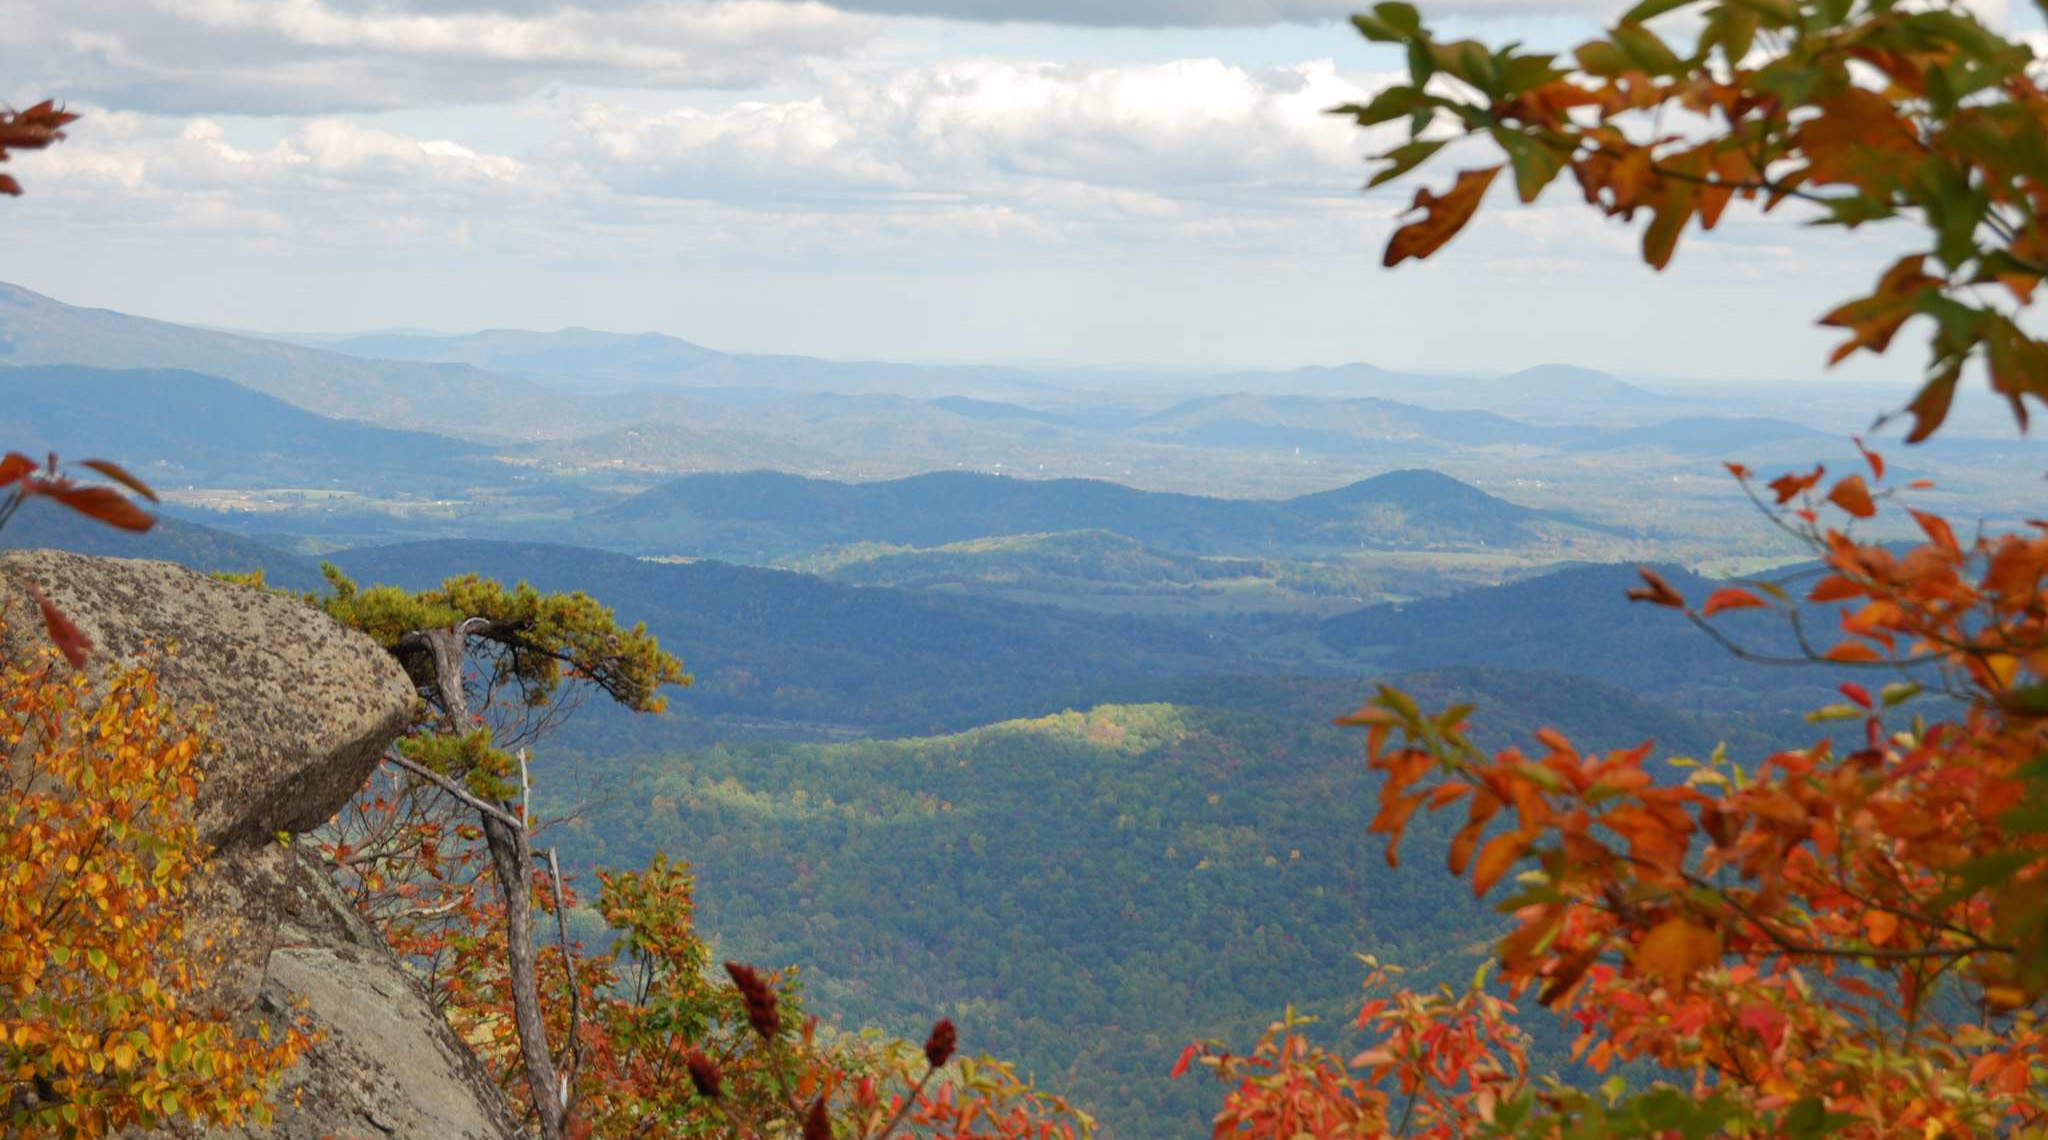
\includegraphics[width=\linewidth]{view}
\caption{Wide Picture}
\label{fig:view}
\end{figure*}

\lipsum[4] % Dummy text

\begin{equation}
\cos^3 \theta =\frac{1}{4}\cos\theta+\frac{3}{4}\cos 3\theta
\label{eq:refname2}
\end{equation}

\lipsum[5] % Dummy text

\subsection{Goal}

\lipsum[6] % Dummy text

\subsection{Global input process output}
some text about the IPO
\paragraph{Paragraph} \lipsum[7] % Dummy text
\paragraph{Paragraph} \lipsum[8] % Dummy text

\subsection{Design specifications}

\paragraph{Functional specifications}
\begin{itemize}[noitemsep] % [noitemsep] removes whitespace between the items for a compact look
	\item First item in a list
	\item Second item in a list
	\item Third item in a list
\end{itemize}

\paragraph{Technical specifications}
\begin{itemize}[noitemsep] % [noitemsep] removes whitespace between the items for a compact look
	\item First item in a list
	\item Second item in a list
	\item Third item in a list
\end{itemize}

\subsection{User interface}
\lipsum[3]
\paragraph{Graphical User Interface}
\lipsum[2]
\paragraph{Hardware User Interface}
\lipsum[1]

\begin{figure}[ht]\centering
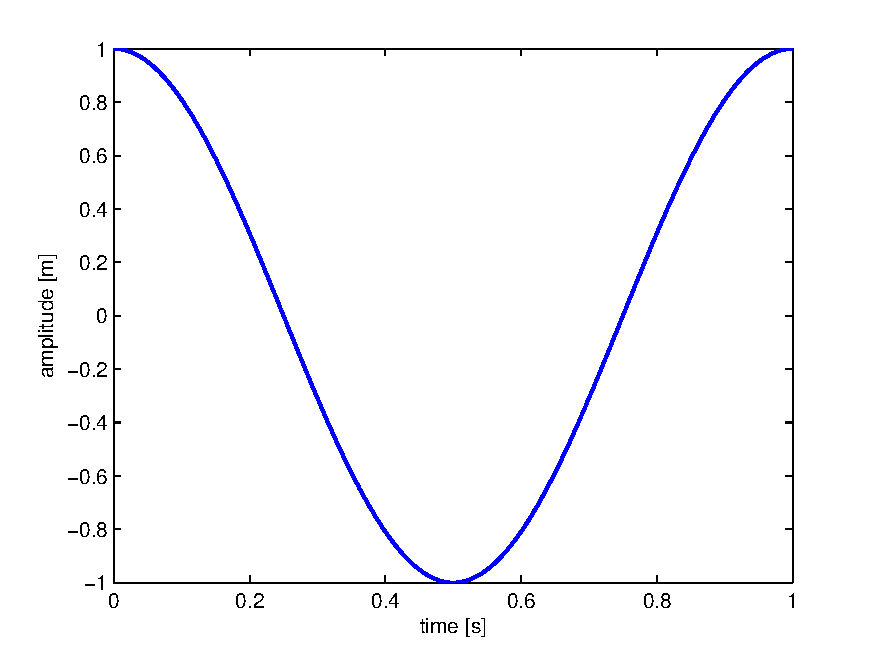
\includegraphics[width=\linewidth]{results}
\caption{In-text Picture}
\label{fig:results}
\end{figure}

\subsection{Manual}
\lipsum[2]
\paragraph{User manual}
\lipsum[4]
\paragraph{Administrator Manual}
\lipsum[6]
Reference to Figure \ref{fig:results}.

%------------------------------------------------

\section{Global Technical design}

\lipsum[10] % Dummy text

\section{Vision Design}

\lipsum[10] % Dummy text

\section{Vision execution}

\lipsum[11] % Dummy text

\subsection{Image acquisition}

\lipsum[12] % Dummy text

\subsection{Image enhancement}

\lipsum[13] % Dummy text


\subsection{Particle segmentation}

\lipsum[14] % Dummy text

\subsection{Feature extraction}

\lipsum[15-23] % Dummy text

%------------------------------------------------
\phantomsection
\section*{Acknowledgments} % The \section*{} command stops section numbering

\addcontentsline{toc}{section}{Acknowledgments} % Adds this section to the table of contents

So long and thanks for all the fish \cite{Figueredo:2009dg}.

%----------------------------------------------------------------------------------------
%	REFERENCE LIST
%----------------------------------------------------------------------------------------
\phantomsection
\bibliographystyle{unsrt}
\bibliography{sample}

%----------------------------------------------------------------------------------------

\newpage
\onecolumn
\appendix
\section{SoilMath Library}
\subsection{Genetic Algorithm Class}
\lstinputlisting[language=C++]{GA.h}
\newpage
\lstinputlisting[language=C++]{GA.cpp}
\newpage
\subsection{Fast Fourier Transform Class}
\lstinputlisting[language=C++]{FFT.h}
\newpage
\lstinputlisting[language=C++]{FFT.cpp}
\newpage
\subsection{Neural Network Class}
\lstinputlisting[language=C++]{NN.h}
\newpage
\lstinputlisting[language=C++]{NN.cpp}
\newpage
\subsection{Statistical Class}
\lstinputlisting[language=C++]{Stats.h}
\newpage
\lstinputlisting[language=C++]{psd.h}
\newpage
\subsection{General project file}
\lstinputlisting[language=C++]{SoilMath.h}
\newpage
\lstinputlisting[language=C++]{CommonOperations.h}
\newpage
\lstinputlisting[language=C++]{SoilMathTypes.h}
\newpage
\lstinputlisting[language=C++]{Mat_archive.h}
\newpage
\lstinputlisting[language=C++]{predict_t_archive.h}
\newpage
\lstinputlisting[language=C++]{MathException.h}
\newpage
\lstinputlisting[language=C++]{Sort.h}

\end{document}